
\chapter{Materiais e Métodos}
\label{chap:mat}

A metodologia empregada para gerenciamento e execução do projeto ELIR é a mesma empregada na área de Robótica da Instituição. O projeto foi divido em três fases principais:

\begin{itemize}
	\item \textit{Conceitual e Design}
	\item \textit{Development}
	\item \textit{Tests}
\end{itemize}

Na etapa de \textit{Conceitual e Design} foram definidos os sensores a serem utilizados no projeto, o modelo esquemático de alimentação e comunicação bem como toda análise de funcionalidades e arquiteturas do robô. Esta é a etapa de criação de conceito tecnológico e o sucesso das demais etapas estão diretamente relacionadas ao sucesso desta.

Na etapa de \textit{Development} as funcionalidades foram implementadas em código e todas as interfaces de alimentação e comunicação foram validadas. Esta fase é marcada pela implementação dos protocolos de comunicação, integração dos sensores com o \textit{framework} de robótica e desenvolvimento da interface gráfica.

Já na etapa \textit{Tests} foram realizados os testes unitários e integrados do sistema de percepção do robô comprovando o seu funcionamento.

%--------- NEW SECTION ----------------------
%\section{Especificação dos componentes}
%\label{sec:espc}
%asjdflkdjsaf

\section{Estrutura analítica do protótipo}
\label{ssec:pbs}
De forma sistemática o projeto ELIR foi dividido em 6 subsistemas, caraterizando a estrutura analítica do projeto (Figura \ref{fig:pbselir}) em:

\begin{itemize}
	\item \textit{perception}
	\item \textit{actuation}
	\item \textit{power management}
	\item \textit{processing system}
	\item \textit{detection}
	\item \textit{software}
\end{itemize}

Os cinco iniciais subsistemas estão mais ligados as condições físicas de hardware do que o subsistema \textit{software}, porém as implicações de software também devem ser consideradas em cada um destes susbsistemas.

O susbistema \textit{software} foi idealizado a partir das funcionalidades desenvolvidas  para a solução final do projeto, e estão descriminadas na secção \ref{sec:espf}.

%----- figure --------------------------------------
\begin{figure}[!htb]
	\centering
	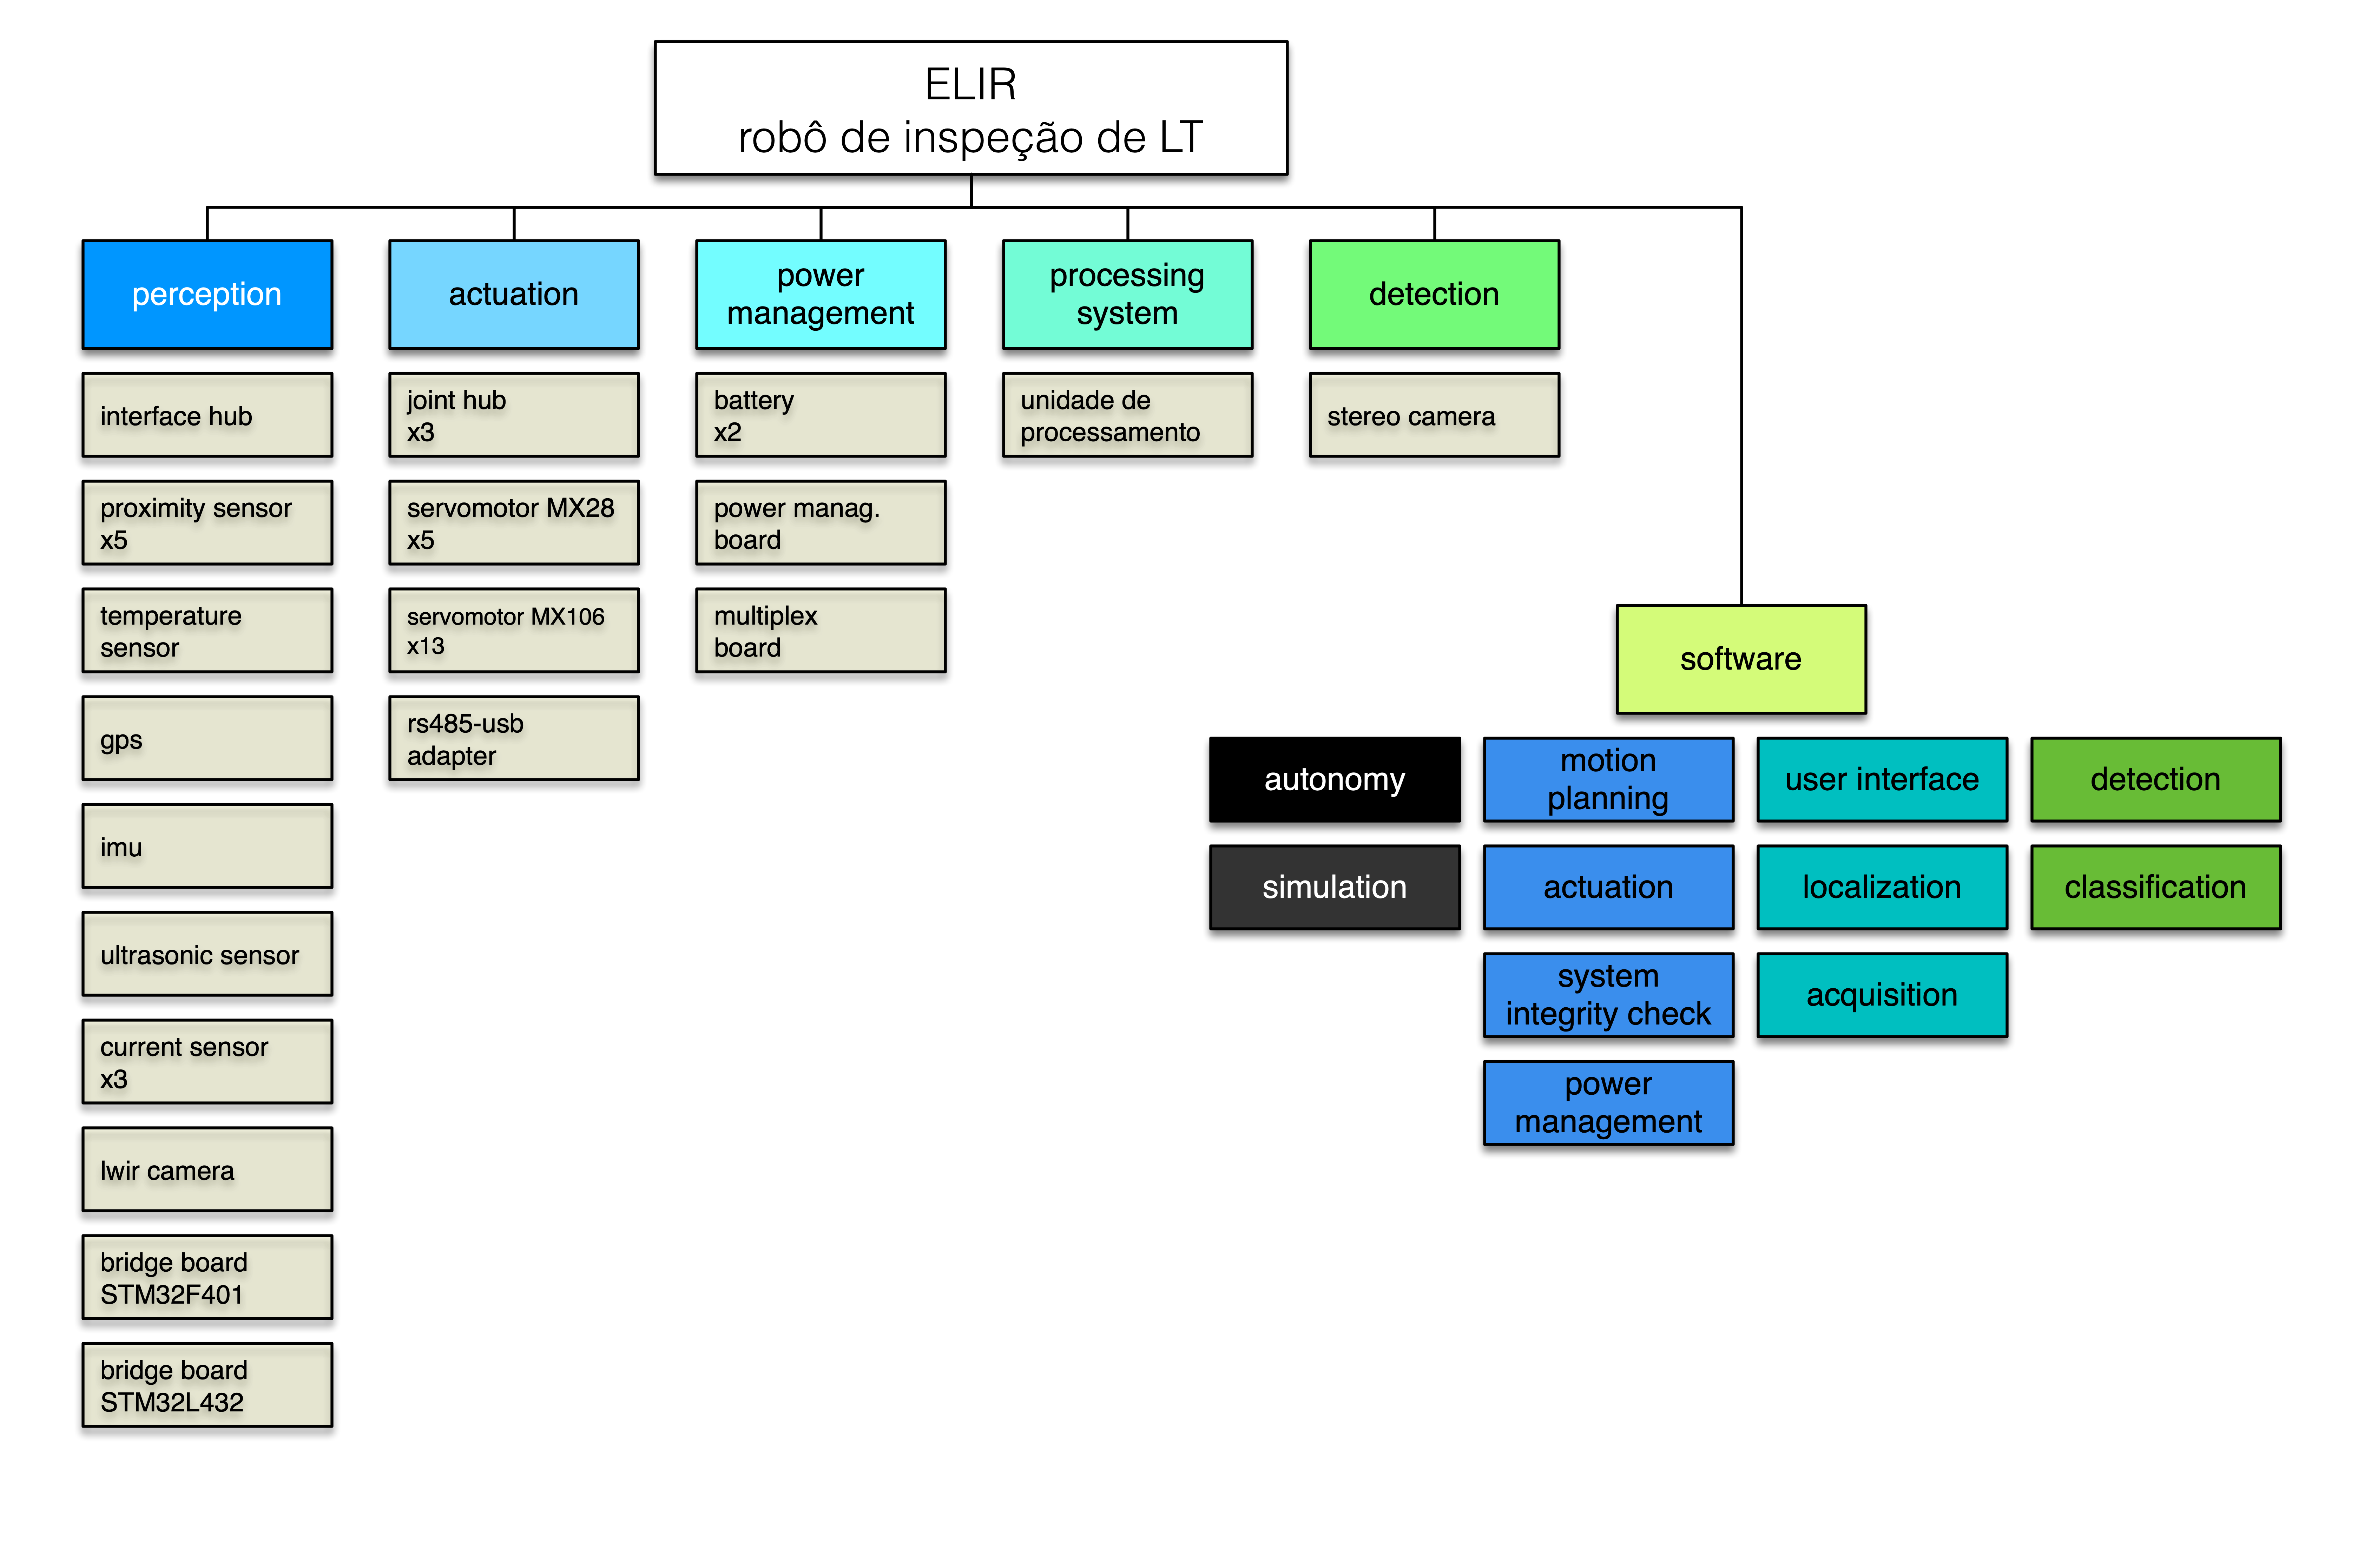
\includegraphics[scale=0.6]{Figures/pbselir.png}
	\caption{Esturutura analítica do sistema.}
	%\legend{Fonte: os autores}
	\label{fig:pbselir}
\end{figure}
%---------------------------------------------------

%fazer comentário sobre os subsistemas

A relação final dos componentes do sistema robótico encontra-se no Apêndice \ref{Append:bom}.


\section{Lista de componentes}
\label{ssec:list}

No sistema de Percepção os sensores atuam como os sentidos do robô, recebendo dados externos e informando a unidade central de processamento os seus significados. Quanto maior o número de grandezas físicas analisadas, mais complexo o sistema de Percepção e maior a sua capacidade de compreensão. 

Os sensores que compõem o sistema de Percepção do robô ELIR foram escolhidos com base nas necessidades de cada funcionalidade do sistema e disponibilidade do componente na própria instituição. A lista de componentes utilizada está mostrada na Figura \ref{fig:list_mat}.

\begin{figure}[h]
	\centering
	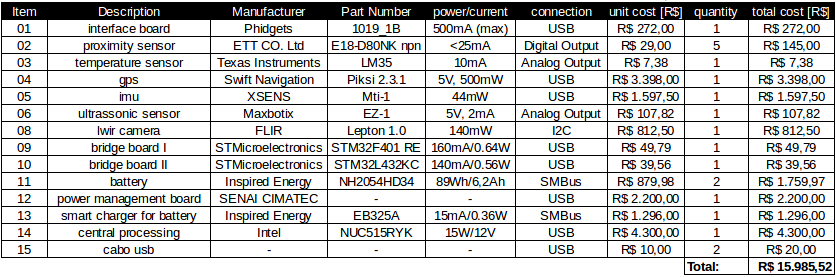
\includegraphics[width=16cm]{Figures/lista_materiais.png}
	\caption{Lista de materiais utilizados no sistema de Percepção do robô ELIR}
	\label{fig:list_mat}
	\source{Própria}
\end{figure}


%--------- NEW SECTION ----------------------
\section{Diagramas mecânicos do sistema de Percepção}
\label{sec:diagm}

O sistema de Percepção em robôs muitas vezes é entendida como uma implementação em código das funcionalidades do sistema, desconsiderando o aporte mecânico envolvido. Contudo, o suporte mecânico para os sensores é um grande desafio a ser solucionado. 

Neste projeto, houve a necessidade de suportes mecânicos por conta da limitação de espaço além de haver uma restrição imposta pelo cliente na modificação estrutural no protótipo. A descrição dos suportes mecânicos desenvolvidos para confrontar esse problema esta mostrada na próxima sessão.
%
%\subsection{Diagrama mecânico do ELIR}
%shaushaus

\subsection{Suporte dos sensores}

Para  fixar  todos  os  sensores  e  componentes  eletrônicos  de  maneira  organizada foi desenhada uma estrutura em forma de prateleira  na qual é possível anexar a grande parte dos sensores do sistema de Percepção.

 A primeira prateleira comporta os sensores do sistema de georreferenciamento que são o GPS e a IMU. A prateleira central foi projetada para a placa de interface Nucleo F401RE que recebe os dados da câmera IR. Por último, na terceira prateleira fica a placa de interface Phidgets para reunir os dados dos diferentes componentes e enviar para a NUC que é a  unidade de processamento central do robô.

As peças foram fabricadas utilizando impressão 3D e o seu desenho pode ser visto nas Figura \ref{Prateleira} e \ref{Prateleiracsensor} .

 \begin{figure}[h]
 	\centering
 	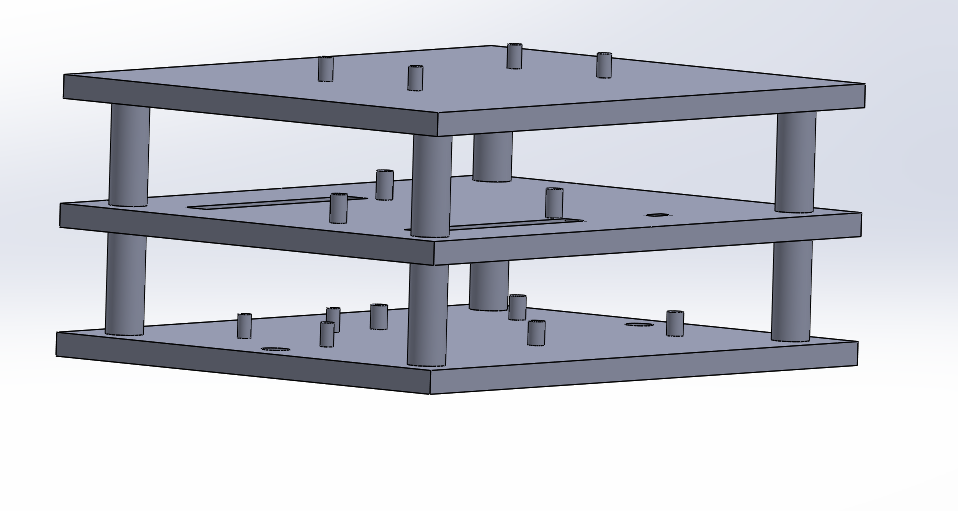
\includegraphics[width=14cm]{Figures/prateleira.png}
 	\caption{Prateleira para suporte dos componentes eletrônicos} \label{Prateleira}
 \end{figure}
 
  \begin{figure}[h]
  	\centering
  	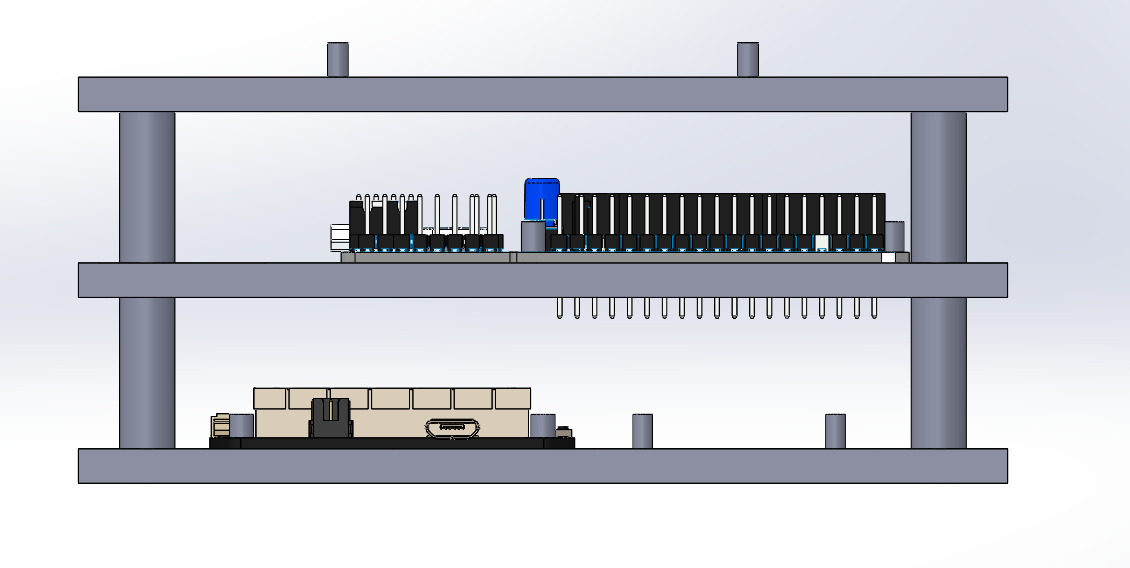
\includegraphics[width=16cm]{Figures/prateleiracsensores.png}
  	\caption{Prateleira para suporte com sensores} \label{Prateleiracsensor}
  \end{figure}
 

A parte de gerenciamento enérgico do robô foi alocada em uma estrutura na parte inferior do mesmo. Esta estrutura foi projetada para comportar as baterias, a \textit{Smart Charger}, a \textit{Power Management} e a placa de interface Nucleo L432. O desenho dessa estrutura está mostrado na figura \ref{pecaaliment}.

\begin{figure}[h]
	\centering
	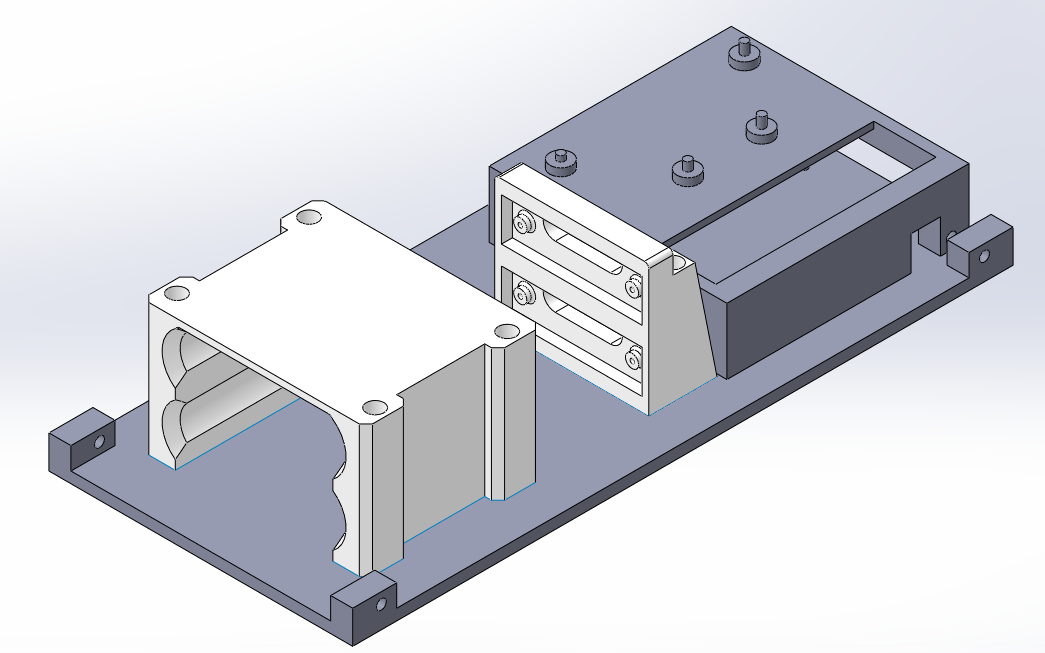
\includegraphics[width=14cm]{Figures/pecadebaixo.png}
	\caption{Prateleira para suporte dos componentes de alimentação} \label{pecaaliment}
\end{figure}

%--------- NEW SECTION ----------------------
\section{Modelo esquemático de alimentação e comunicação}
\label{sec:modesq}

A alimentação do sistema é proveniente de duas baterias LiPo que fornecem tensão de alimentação em 14V. Todo o gerenciamento de energia do sistema é feita pela \textit{Power Management Board}, esta placa é responsável por distribuir a alimentação de entrada para os demais subsistemas da Percepção. 

A placa de interface Phidgets além de funcionar como \textit{hub} para uma grande parte dos sensores também é responsável por compatibilizar o nível de tensão para os componentes eletrônicos, fornecendo 5V para as placas microprocessadas, sensores e a alimentação de todas as portas USBs. 

A comunicação entre os sistemas da Percepção ocorrem na maior parte  através da Phidgets, já que esta placa de interface concentra as informações oriundas de suas portas USB, entrada digitais e entradas analógicas em uma única porta USB para a unidade central de processamento.

 A câmera térmica e a os dynamixels possuem portas exclusivas de comunicação com a unidade central devido seu grau de criticidade.

\subsection{Diagramas elétricos e eletrônicos}
\label{sec:diage}
O diagrama elétrico do sistema está disponível no apêndice \ref{Append:diagele}. Neste diagrama encontram-se todas as conexões elétricas e de comunicação bem como as especificações de conectores e cabos utilizados no projeto.

O esquemático eletrônico realizado pela equipe foi uma placa hub de 5V para alimentação dos sensores de proximidade, visto que a Phidgets possui apenas umas saída de tensão em 5V disponibilizada.

 Nesta placa foram colocados os \textit{pin headers} para cada sensor de proximidade, fornecendo alimentação e disponibilizando os pinos digitais dos sensores em um conector Molex.

O esquemático eletrônico e \textit{board} estão mostrados no anexo \ref{Append:diagele}.


%--------- NEW SECTION ----------------------
\section{Especificação das funcionalidades}
\label{sec:espf}
Diante da arquitetura apresentada anteriormente e focando nos objetivos traçados no Capítulo \ref{chap:intro}, o sistema robótico foi dimensionado para onze funcionalidades distintas:

\begin{enumerate}%[itemsep=1pt]
	%\setlength\itemsep{1em}
	\item sistema de verificação da integridade
	\item gerenciamento de energia
	\item aquisição
	\item localização
	\item planejamento de movimento
	\item atuação
	\item detecção
	\item classificação
	\item interface do usuário
	\item autonomia
	\item simulação
\end{enumerate}

A Figura \ref{img:elirfluxo} apresenta o fluxo de informações entre as funcionalidades. Este fluxo deve ser compreendido para que seja estabelecida as relações entre as funcionalidades e o entendimento entre elas, essa compreensão impactará na melhor elaboração da árvore de falhas do sistema e proporcionará um sistema mais confiável.

%---------------picture------------------------------------
\begin{figure} [h!]	
	\caption{Fluxo de informações do sistema.}
	\label{img:elirfluxo}											 
	\centering													 
	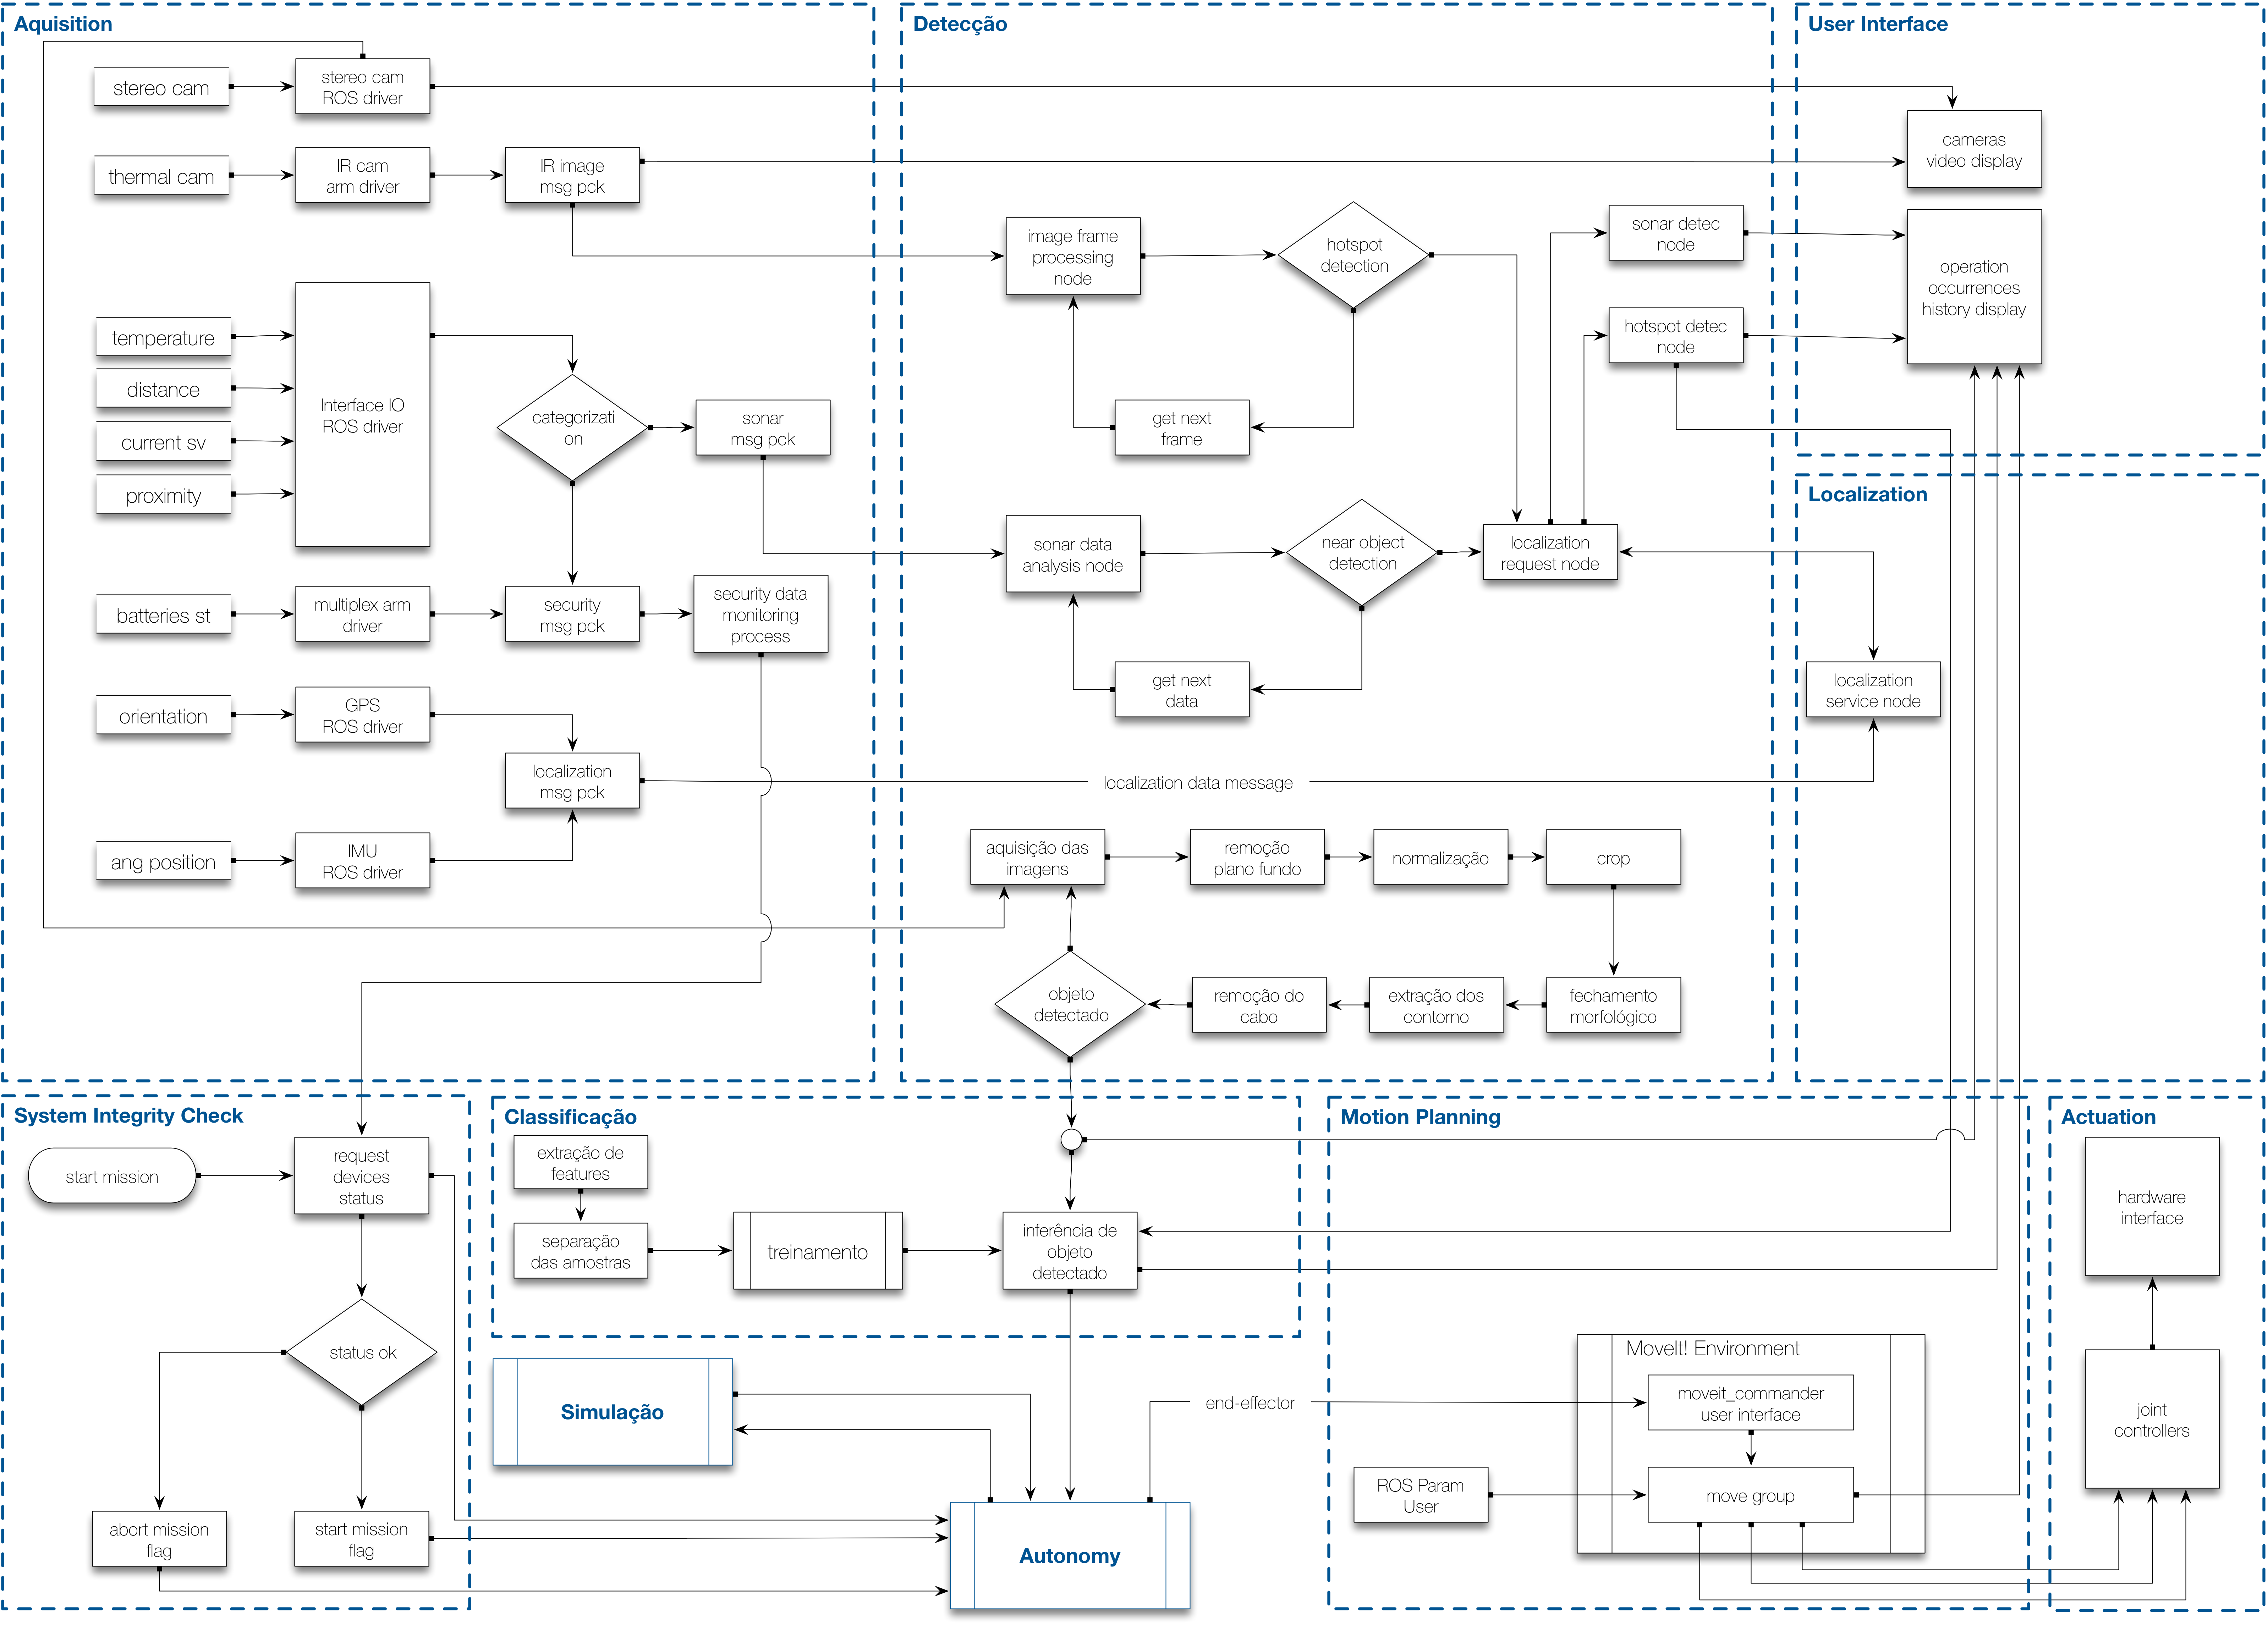
\includegraphics[width=1.0\textwidth]{Figures/flxinfofunctionalities}
	%\fautor			 											 
\end{figure}													 
%----------------------------------------------------------

Nas seções seguintes são apresentados em maiores detalhes sobre cada uma das funcionalidades do sistema robótico. Para que fosse melhor compreendido, o desenvolvimento destas funcionalidades foram agrupadas em cinco áreas: movimentação, percepção, interface do usuário, autonomia e simulação. As duas áreas iniciais foram subdivididas em planejamento de movimento, sistema de verificação de integridade, atuação e gerenciamento de energia para a primeira área de nome \textbf{movimentação}, que tem como principal objetivo garantir a execução da missão e transposição de obstáculos. Para a segunda área, nominada por percepção, a subdivisão ficou da seguinte forma: aquisição, detecção, classificação e localização, que como o significado do próprio nome apresenta como objetivo principal a percepção do robô diante do ambiente inserido.

\subsection{Fluxo das informações do sistema de Percepção}
\label{ssec:fluxo}


As funcionalidades de um robô descrevem os subsistemas e a lógica de operação dos mesmos. No ELIR, o sistema de Percepção possui três funcionalidades principais: Aquisição, Localização e Detecção. A descrição de cada funcionalidade e seu diagrama de funcionamento estão mostrados nos subtópicos a seguir. 

\subsection{Aquisição}
\label{ssec:func1}

O processo de aquisição de dados envolve a comunicação dos sensores com seus respectivos drivers no ambiente ROS e a disponibilização dos dados para as outras funcionalidades do sistema.

 Os sensores analógicos e digitais terão seus dados tratados pelo driver da interface Phidgets no ambiente ROS. Para os dispositivos relacionados a localização como o GPS e a IMU, serão utilizado drivers já disponibilizados pelos fabricantes.

No caso dos componentes que trabalham com os protocolos de comunicação SPI ou I2C, como é o caso da câmera térmica e da \textit{Smart Charger}, serão utilizadas duas interfaces baseadas em ARM com um \textit{firmware} embarcado para a conversão dos dados para o protocolo UART.

A interface microprocessada utilizada para obter dados da câmera térmica possui uma porta USB dedicada na unidade de processamento Intel NUC. Já a outra interface microprocessada para a \textit{Smart Charger} será conectada a uma porta USB da Phidgets.

No ambiente ROS do projeto há um \textit{package} exclusivo para receber os dados convertidos da câmera térmica, um \textit{package} para receber dados de todos os sensores conectados a Phidgets, um \textit{package} para recebimento de dados da \textit{Smart Charger} e por último um \textit{package} exclusivo para interface gráfica. 
Pode-se observar o fluxograma da aquisição na Figura \ref{FuncAquisition}

\begin{figure}[!ht]
	\centering
	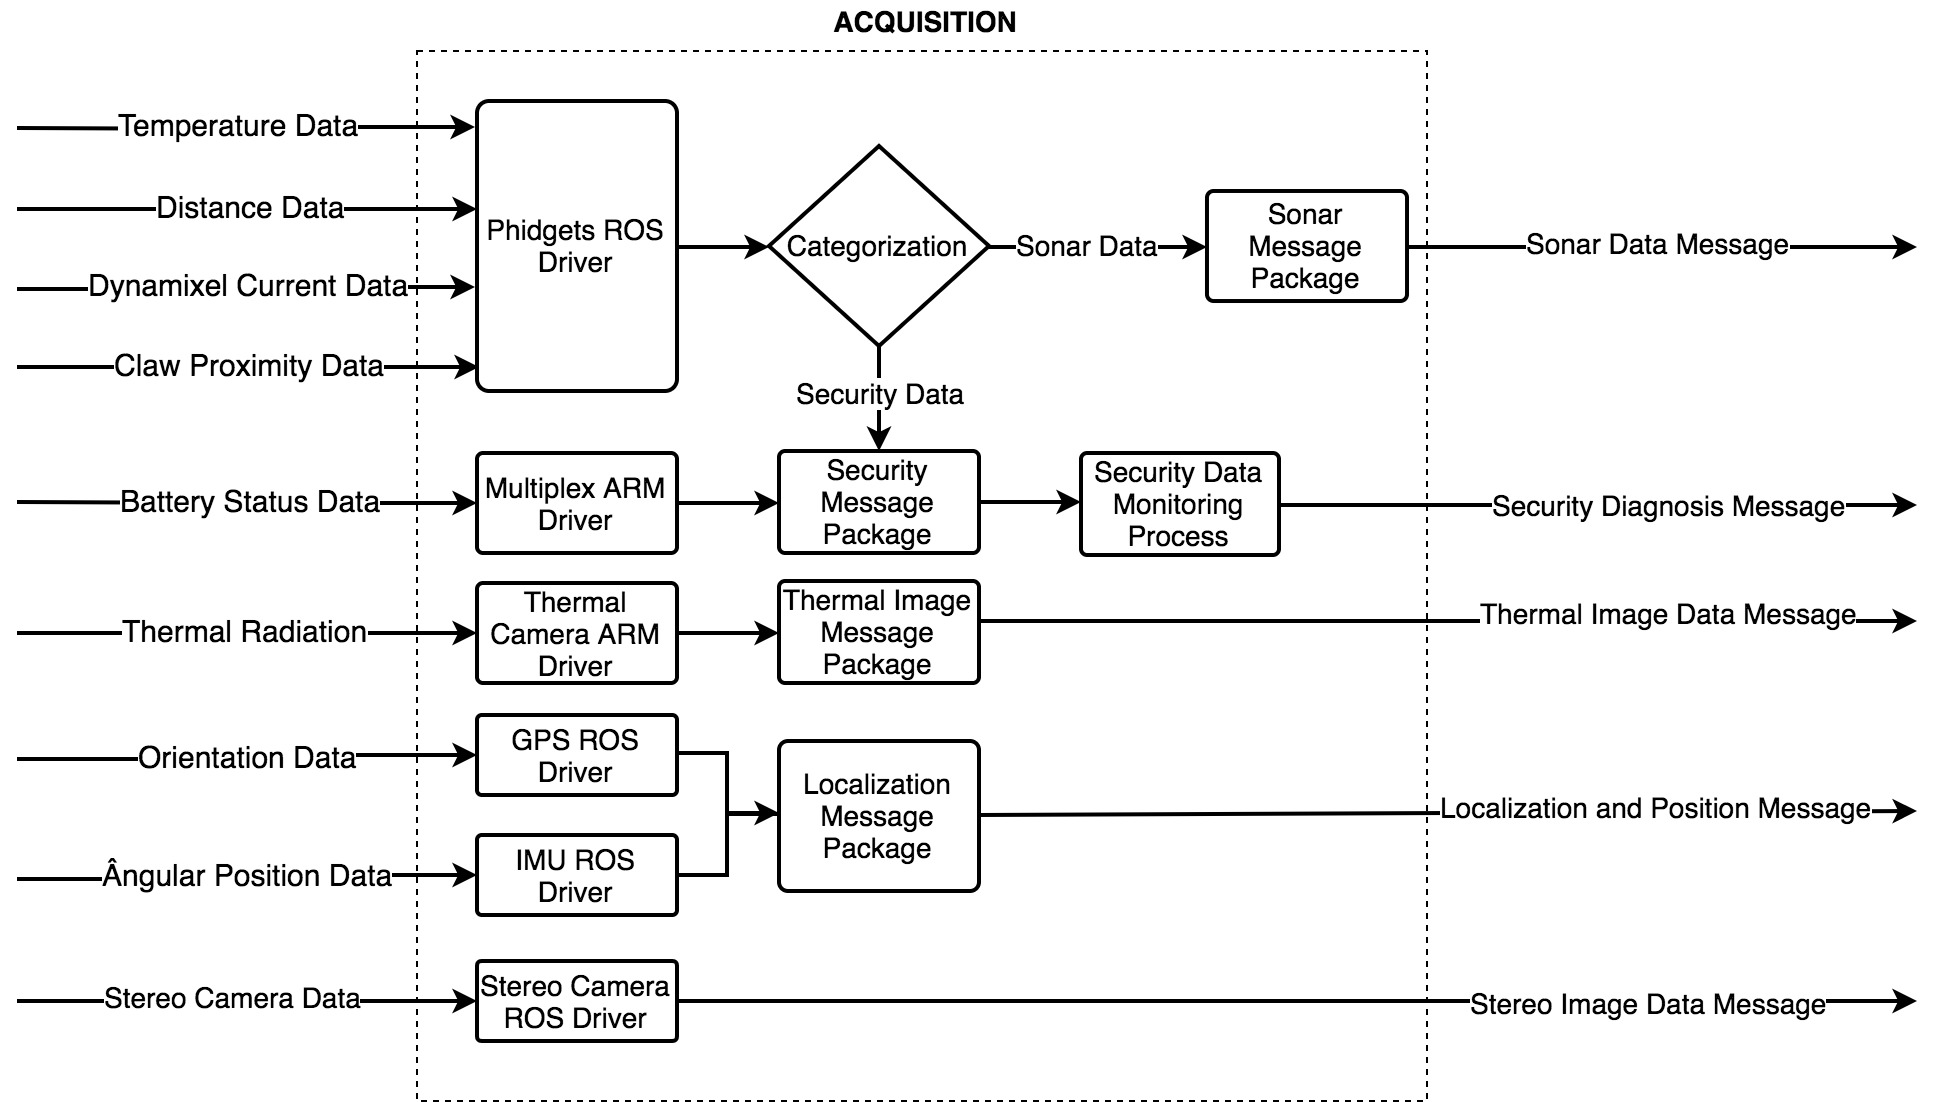
\includegraphics[height=7cm, width=14cm]{Figures/Fluxograma_Aquisition.jpg}
	\caption{Fluxograma da Funcionalidade Aquisição} \label{FuncAquisition}
\end{figure}

Para correta execução desta funcionalidade é necessário o funcionamento dos sensores segundo o nível de prioridade dos mesmos. Logo, um estudo de casos de falhas para cada sensor foi realizado, no qual foi definido um nível de criticidade de acordo com o impacto de sua função no sistema como um todo. Foram elaborados três níveis de criticidade:
\begin{itemize}
	\item Level 1 - Sensores com impacto crítico na operação. Em casos de falha, a inspeção não poderá ser realizada.
	\item Level 2 - Sensores com impacto médio na operação. Em caso de falha, a inspeção poderá ser realizada de forma parcial.
	\item Level 3 - Sensores com impacto leve na operação. Em caso de falha, não haverá dados de monitoramento da situação de temperatura e consuno energético do robô, porém a inspeção poderá continuar normalmente.
\end{itemize}

Na figura abaixo, pode-se observar os sensores e suas categorias.

\begin{figure}[!ht]
	\centering
	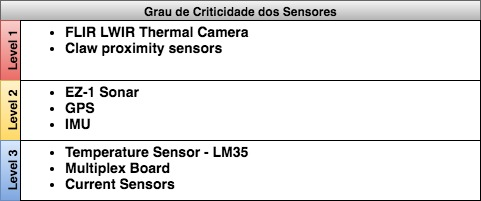
\includegraphics[height=7cm, width=14cm]{Figures/criticidade.jpg}
	\caption{Nível de criticidade dos sensores} \label{FuncAquisition}
\end{figure}

\subsubsection{Objetivo}
Realizar a comunicação e a aquisição dos dados provenientes da câmera térmica, sensores de proximidade, sonar, GPS, IMU, sensor de temperatura, \textit{Smart Charger} e sensores de corrente.

\subsubsection{Dependências}
Esta funcionalidade não é dependente de nenhum outro processo.

\subsubsection{Premissas}
\begin{itemize}
	\item A interface microcontrolada Nucleo STM32F401RE deve estar com firmware embarcado para conversão de dados SPI para UART.
	\item A câmera térmica deverá estar conectada à interface Nucleo STM32F401RE
	\item A câmera stereo deve está conectada à NUC através da porta USB
	\item O sensores de temperatura, corrente e sonar devem estar conectados as entradas analógicas da interface Phidgets
	\item Os sensores de proximidade devem está conectados as entradas digitais da placa de interface Phidgets
	\item O GPS e a IMU devem estar conectados a portas USB da Phidgets
	\item As placas de interface devem estar energizadas.
\end{itemize}

\subsubsection{Saídas}

Esta funcionalidade possui quatro saídas:

\begin{itemize}
	\item \textit{Sonar Data Message}: Mensagem de saída exclusiva para os dados do sonar EZ-1.
	\item \textit{Secutiry Diagnose Message}: Mensagem contendo todos os dados relacionados à segurança e integridade do robô.
	\item \textit{Thermal Image Data Message}: Mensagem exclusiva para os dados da câmera térmica.
	\item \textit{Localization and Position Message}: Mensagem contendo os dados relacionados á localização e posicionamento angular do robô.
\end{itemize}

\subsection{Localização}
\label{ssec:func2}

O sistema de localização envolve o monitoramento da posição latitudinal e longitudinal do robô, assim como a posição angular através do GPS e da IMU respectivamente.

A localização é um package que ao receber uma requisição de informação, coleta os dados de posicionamento e orientação do robô provenientes do sistema de Aquisição e encaminha para o sistema que requisitou.

O fluxograma deste funcionalidade pode ser visto na Figura \ref{fluxlocal}

\begin{figure}[h!]
	\centering
	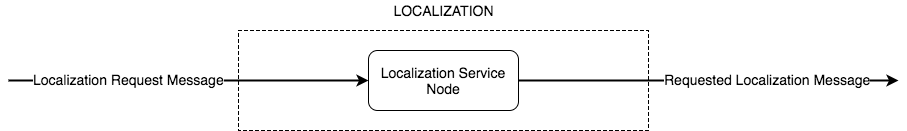
\includegraphics[width=16cm]{Fluxograma_Localization.png}
	\caption{Fluxograma da Funcionalidade Localização} \label{fluxlocal}
\end{figure}


\subsubsection{Objetivo}
O objetivo desta funcionalidade é disponibilizar os dados de Localização do robô no ambiente ROS para a funcionalidade de Detecção.

\subsubsection{Dependências}
O sistema de localização depende dos dados de posicionamento e orientação disponibilizados pelo sistema de Aquisição.

\subsubsection{Premissas}
\begin{itemize}
	\item O sistema de Aquisição deve está funcionando corretamente até o Nível 2 de criticidade dos sensores.
	\item GPS e IMU estão posicionados em uma estrutura rígida e com o menor vibração possível.
\end{itemize}

\subsubsection{Saídas}

\begin{itemize}
	\item \textit{Requested Localization Message}: Mensagem que informa os dados de localização para o sistema que os requisitou.
\end{itemize}

\subsection{Detecção}
\label{ssec:func3}

A detecção é a funcionalidade responsável por identificar a presença de pontos quentes na linha de transmissão bem como de objetos na faixa de servidão. Ao identificar um destes elementos, o sistema solicita da funcionalidade de Localização os dados posicionamento e orientação do robô e envia uma mensagem de alerta.

A mensagem de detecção de um ponto quente informa a localização do robô e a localização do objeto no frame de imagem. Por isso recebe a mensagem de detecção de obstáculos. 

A mensagem de detecção de objetos na faixa de servidão informa a distância da cota da linha até o objeto e a localização do mesmo. 

\subsubsection{Objetivo}

O objetivo desta funcionalidade é coletar as informações provenientes da câmera infravermelha e do sonar, como presença de pontos quentes e objetos presentes na área de servidão. 

\subsubsection{Dependências}
O sistema de detecção depende dos dados do sonar e dos \textit{frames} da câmera térmica disponibilizados pelo sistema de Aquisição. Além disto, depende do sistema de Localização para adquirir informações de posicionamento e orientação do robô.

\subsubsection{Premissas}
\begin{itemize}
	\item O sistema de Aquisição deve está funcionando corretamente até o Nível 2 de criticidade dos sensores.
	\item A câmera térmica deve estar calibrada e posicionada com ângulo de visão para as linhas de transmissão e seus obstáculos
	\item O sonar deve estar posicionado de forma a monitorar objetos abaixo da linha de transmissão.            
\end{itemize}

\begin{figure}[!ht]
	\centering
	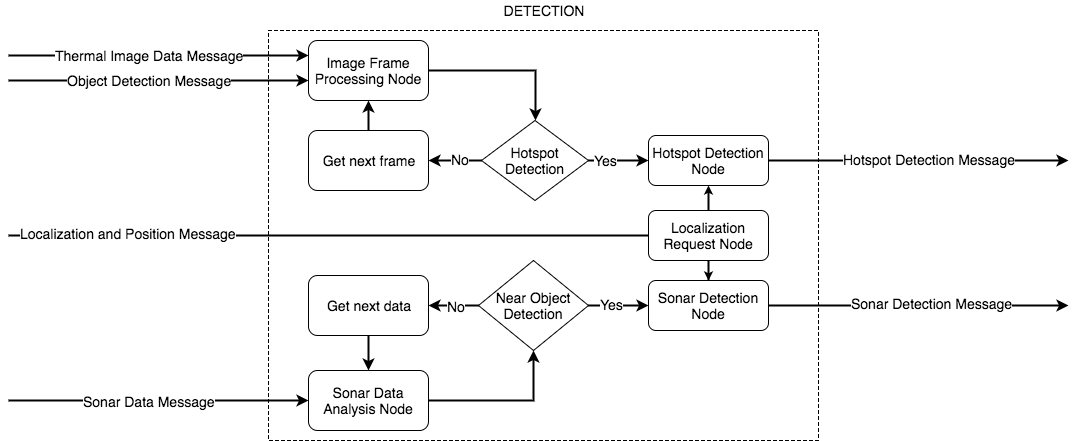
\includegraphics[width=16cm]{Fluxograma_Detection.png}
	\caption{Fluxograma da Funcionalidade Detecção} \label{FuncDetec}
\end{figure}

\subsubsection{Saídas}

\begin{itemize}
	\item \textit{Hotspot Detection Message}: Mensagem que informa a detecção de um ponto quente e informa a sua localização na imagem e localização do robô na linha.
	\item \textit{Sonar Detection Message}: Mensagem que informa a detecção de objetos na faixa de servidão e sua localização na linha.
	%\item Localization Request Message: Mensagem de requisição dos dados posicionamento e orientação do robô para o sistema de Localização
\end{itemize}


%--------- NEW SECTION ----------------------
\section{Interface do Usuário}
\label{sec:ui}

A interface do usuário é uma forma de expor graficamente as variáveis mais importantes do sistema robótico e quais atividades estão sendo executadas. Ela permite dar previsibilidade ao usuário do comportamento do sistema. 

No ELIR a interface do usuário tem o papel de informar cinco características principais:

\begin{itemize}
	\item \textit{System Integrity}
	\item \textit{Robot Status}
	\item \textit{Thermal view}
	\item \textit{Ocurrences}
	\item \textit{Actuators Information}
\end{itemize}

No campo de \textit{System Integrity} são exibidos em tempo real as variáveis de grande impacto na eficiência e integridade do sistema. Por isso são informados os dados de temperatura, percentual de carga da bateria, consumo, localização e orientação do robô.

O \textit{Robot Status Display} exibe o posicionamento das garras do robô na linha de transmissão. A coloração vermelha indica as garras foras da linha enquanto que a coloração verde indica as garras apoiadas na linha. Essa informação proveniente dos sensores de proximidade é de extrema importância para integridade física do robô.

O \textit{Thermal View} exibe em  tempo real os frames da câmera IR, permitindo o usuário acompanhar a detecção de pontos quentes e visualizar o perfil de temperatura da área exibida. 

O campo de \textit{Ocurrences} mostra as principais ocorrências daquele momento, mostrando eventos de sobretemperatura, sobrecorrente, detecção de pontos quentes e detecção de objetos na área de servidão. Todos os eventos são mostra
dos com data, horário e localização gps. 


%\begin{figure}[!ht]
%	\centering
%	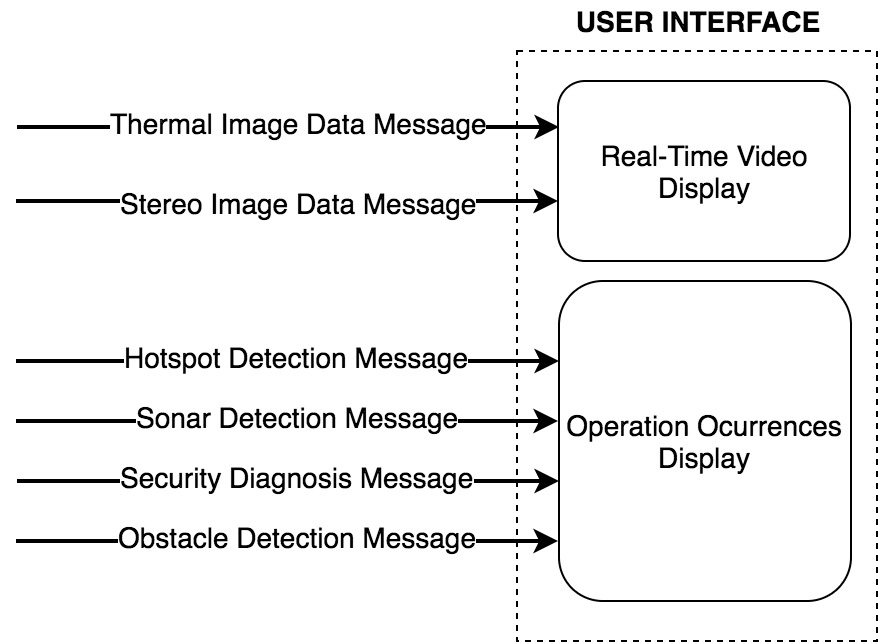
\includegraphics[width=14cm]{Figures/Fluxograma_Interface.jpg}
%	\caption{Fluxograma da Interface do Usuário} \label{UI}
%\end{figure}
